%%%%%%%%%%%%%%%%%%%%%%%%%%%%%%%%%%%%%%%%%%%%%%%%%%%%%%%%%%%%%%%%%%%%
%% I, the copyright holder of this work, release this work into the
%% public domain. This applies worldwide. In some countries this may
%% not be legally possible; if so: I grant anyone the right to use
%% this work for any purpose, without any conditions, unless such
%% conditions are required by law.
%%%%%%%%%%%%%%%%%%%%%%%%%%%%%%%%%%%%%%%%%%%%%%%%%%%%%%%%%%%%%%%%%%%%

\documentclass{beamer}
\usetheme[faculty=fi]{fibeamer}
\usepackage[utf8]{inputenc}
\usepackage[
  main=english, %% By using `czech` or `slovak` as the main locale
                %% instead of `english`, you can typeset the
                %% presentation in either Czech or Slovak,
                %% respectively.
  czech, slovak %% The additional keys allow foreign texts to be
]{babel}        %% typeset as follows:
%%
%%   \begin{otherlanguage}{czech}   ... \end{otherlanguage}
%%   \begin{otherlanguage}{slovak}  ... \end{otherlanguage}
%%
%% These macros specify information about the presentation
\title{Lightweight Gate Detection for Autonomous Drone Racing} %% that will be typeset on the
\subtitle{Mid-Term Presentation} %% title page.
\author{Philipp Dürnay}
%% These additional packages are used within the document:
\usepackage{ragged2e}  % `\justifying` text
\usepackage{booktabs}  % Tables
\usepackage{tabularx}
\usepackage{tikz}      % Diagrams
\usetikzlibrary{calc, shapes, backgrounds}
\usepackage{amsmath, amssymb}
\usepackage{url}       % `\url`s
\usepackage{listings}  % Code listings
\frenchspacing
\begin{document}
  \frame{\maketitle}

  \AtBeginSection[2,3,4]{% Print an outline at the beginning of sections
    \begin{frame}<beamer>
      \frametitle{Outline for Section \thesection}
      \tableofcontents[currentsection]
    \end{frame}}

  \begin{darkframes}
  	\begin{frame}{Outline}
  		\tableofcontents
  	\end{frame}
    \section{Background}
    \subsection{Application}
    \begin{frame}{IROS2018}
    	content...
    \end{frame}
    \begin{frame}{Training Data}
       	content...
    \end{frame}
	\subsection{Research Question}    
	\begin{frame}{Research Question}
	\textbf{How can we efficiently detect objects that are largely occupied by backround}, when there is only little amount of training data and the computational resources are limited?
	\end{frame}
    \subsection{Object Detection}
    \begin{frame}{Object Detection}
    	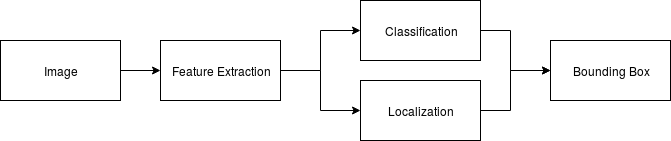
\includegraphics[width=\linewidth]{resources/ObjectDetection}
    \end{frame}
    \begin{frame}{Convolutional Networks}
	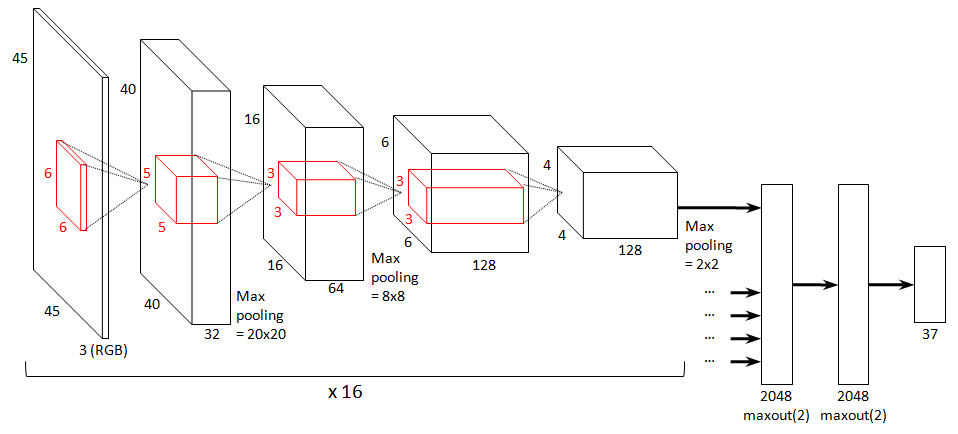
\includegraphics[width=\linewidth]{resources/cnn}
    \end{frame}
    \begin{frame}{One Stage Detectors}
       	content...
    \end{frame}

        
    \section{Proposed Method}
    \begin{frame}{Architecture}
    	content...
    \end{frame}
    
    \section{Evaluation}
    \begin{frame}{Results}
    	content...
    \end{frame}
    
    \section{Conclusion}
    \subsection{Conclusion}
    \begin{frame}{Conclusion}
    	content...
    \end{frame}
    \subsection{Next Steps}
    \begin{frame}{Next Steps}
    	content...
    \end{frame}
    
    \section{Questions}
    \begin{frame}{Questions}
    	content...
    	\end{frame}
    
    
  \end{darkframes}

\end{document}
